\documentclass[11pt,a4paper]{article}

\usepackage[T1]{fontenc}
\usepackage[utf8]{inputenc}
\usepackage{lmodern}
\usepackage[margin=1in]{geometry}
\usepackage{amsmath,amssymb,amsfonts,amsthm,bm}
\usepackage{graphicx}
\usepackage{booktabs}
\usepackage{longtable}
\usepackage{tabularx}
\usepackage{array}
\usepackage{enumitem}
\usepackage{caption}
\usepackage{subcaption}
\usepackage{xcolor}
\usepackage{fancyhdr}
\usepackage{microtype}
\usepackage[round,authoryear]{natbib}
\usepackage[hidelinks]{hyperref}
\usepackage{verbatim}
\usepackage{tikz}
\usetikzlibrary{arrows.meta,positioning,fit,backgrounds}

\newcommand{\paperversion}{1.0.0}
\newcommand{\codecommit}{\texttt{ef13675}}
\newcommand{\evidencetag}{\texttt{final-\allowbreak audit-\allowbreak 2026-10-\allowbreak 31-\allowbreak dpa}}
\newcommand{\F}{\mathbb{F}}
\newcommand{\bits}{\{0,1\}}
\newcommand{\Rec}{\mathsf{Rec}}
\newcommand{\Share}{\mathsf{Share}}
\newcommand{\HW}{\mathsf{HW}}
\newcommand{\Sbox}{\mathsf{SBOX}}
\newcommand{\code}[1]{\texttt{#1}}
\newcommand{\Adv}{\mathcal{A}}
\newcommand{\E}{\mathbb{E}}
\newcommand{\Prb}{\Pr}

\theoremstyle{plain}
\newtheorem{theorem}{Theorem}[section]
\newtheorem{lemma}[theorem]{Lemma}
\newtheorem{proposition}[theorem]{Proposition}
\newtheorem{corollary}[theorem]{Corollary}
\theoremstyle{definition}
\newtheorem{definition}[theorem]{Definition}
\newtheorem{assumption}[theorem]{Assumption}
\newtheorem{claim}[theorem]{Claim}
\theoremstyle{remark}
\newtheorem{remark}[theorem]{Remark}

\newcounter{algblock}
\newenvironment{algorithmblock}[1]{%
  \par\medskip\refstepcounter{algblock}%
  \noindent\textbf{Algorithm \thealgblock} --- #1\par\nopagebreak
  \noindent\begin{minipage}{\linewidth}\small
}{%
  \end{minipage}\par\medskip
}

\pagestyle{fancy}
\fancyhf{}
\fancyhead[L]{\small SiCaS White Paper}
\fancyhead[R]{\small Version \paperversion}
\fancyfoot[C]{\small\thepage}
\renewcommand{\headrulewidth}{0.4pt}

\hypersetup{
  pdftitle={SiCaS: Safe-Rust Side-Channel Attenuation and Leakage Assessment -- White Paper},
  pdfauthor={SiCaS Contributors},
  pdfsubject={Side-channel attenuation and leakage assessment},
  pdfkeywords={side-channel analysis, Boolean masking, TVLA, CPA, DPA, ChaCha20, Rust, reproducible research},
  colorlinks=true,
  linkcolor=blue!45!black,
  citecolor=blue!45!black,
  urlcolor=blue!45!black
}

\title{%
  \vspace{-1.2cm}
  {\LARGE\bfseries SiCaS}\\[0.35cm]
  {\Large Safe-Rust Side-Channel Attenuation and Leakage Assessment}\\[0.25cm]
  {\large White Paper}
}
\author{SiCaS Contributors}
\date{Version \paperversion \quad 31 October 2026}

\setlength{\emergencystretch}{2em}

\begin{document}

\maketitle
\thispagestyle{empty}

\begin{center}
\begin{tabular}{@{}ll@{}}
\toprule
Document & White paper \\
Version & \paperversion \\
Date & 31 October 2026 \\
Code commit & \codecommit \\
Release build commit & \texttt{123eb69} \\
Evidence tag & \evidencetag \\
Public label & SAL-2 locally \\
Production status & Not certified, not audited, not hardware-validated \\
License & GPL-3.0-only \\
\bottomrule
\end{tabular}
\end{center}

\begin{abstract}
Side-channel leakage is a practical threat to implementations of cryptographic
algorithms: power consumption, electromagnetic radiation, and execution time can reveal
information about secret keys even when the algorithm is mathematically secure. SiCaS is
a safe-Rust, zero-runtime-dependency workspace that combines first-order Boolean-masked
primitives and a masked ChaCha20 reference integration with a leakage-assessment
harness for TVLA, CPA, DPA, and timing analysis. This white paper explains the problem,
the threat model, the architecture, the masking construction, the assessment
methodology, the evidence package, and the limitations of the current release. The
project is deliberately local-first and evidence-first: every security claim is mapped
to a proof obligation, a test, a measurement, or a documented limitation. The current
public label is SAL-2 locally; the package is audit-ready but has not been independently
audited, red-teamed, or validated on physical hardware. The paper is therefore both a
technical overview and a precise statement of what the current evidence does and does
not support.
\end{abstract}

\vspace{0.3cm}
\noindent\textbf{Keywords:} side-channel analysis, Boolean masking, TVLA, CPA, DPA,
ChaCha20, safe Rust, reproducible builds, assurance.

\newpage
\tableofcontents
\newpage

\section{Executive summary}

SiCaS addresses two problems that are usually handled by separate teams and separate
toolchains:

\begin{enumerate}[leftmargin=1.5em]
  \item \textbf{Attenuation.} How can cryptographic software be structured so that
        first-order power or electromagnetic leakage is reduced, and how can the
        masking construction be made explicit and reviewable?
  \item \textbf{Assessment.} How can raw power or electromagnetic traces be analysed
        reproducibly, with a clear leakage model, published parameters, and evidence
        that can be independently checked?
\end{enumerate}

The project keeps both sides in one workspace. The \code{sicas-core} crate provides
constant-time primitives, an opaque \code{Secret<T>} wrapper, two-share Boolean masking,
and a masked adder. The \code{sicas-reference} crate exercises those gadgets in a
first-order masked ChaCha20 implementation, including a 64-block bitsliced batch path.
The \code{sicas-harness} crate provides a strict trace format, preprocessing, TVLA, CPA,
AES S-box DPA, dudect-style timing checks, and synthetic validation. The
\code{sicas-platform} crate supplies a fail-closed OS entropy adapter. The
\code{sicas-zeroize} crate is an isolated, non-published, unaudited experiment in
volatile zeroization.

The main contributions of the current release are:

\begin{itemize}[leftmargin=1.5em]
  \item a safe-Rust, zero-runtime-dependency implementation of the core masking and
        constant-time building blocks;
  \item a masked ChaCha20 reference integration with RFC~8439 validation and a
        differential test against an unmasked reference;
  \item a 64-block bitsliced batch path that meets the project's 10$\times$ hard
        performance ceiling;
  \item a leakage-assessment harness covering TVLA, CPA, DPA, timing, preprocessing,
        and synthetic validation;
  \item a formalised claim and proof-obligation structure, a reproducible evidence
        bundle, and a local proof runner;
  \item a precise assurance statement: \textbf{SAL-2 locally}, not SAL-3 or SAL-4.
\end{itemize}

The paper is organised as follows. Section~\ref{sec:intro} introduces the problem and
contributions. Section~\ref{sec:background} reviews side-channel analysis and masking.
Section~\ref{sec:threat} states the threat model. Section~\ref{sec:architecture}
describes the architecture. Section~\ref{sec:design} explains the masking and
cryptographic design. Section~\ref{sec:assessment} describes the leakage-assessment
methodology. Section~\ref{sec:claims} maps claims to evidence.
Section~\ref{sec:implementation} discusses implementation and release engineering.
Section~\ref{sec:evaluation} summarises the evaluation. Section~\ref{sec:limitations}
states the limitations. Section~\ref{sec:roadmap} gives the roadmap to SAL-4.
Section~\ref{sec:related} discusses related work, and Section~\ref{sec:conclusion}
concludes. Appendices provide a glossary, a claim-to-evidence matrix, reproducibility
commands, and the document history.

\section{Introduction}\label{sec:intro}

\subsection{Motivation}

A cryptographic implementation can be mathematically secure and still leak its key
through its physical behaviour. Kocher's timing attack \citep{kocher1996timing} showed
that data-dependent execution time can reveal secret information. Differential power
analysis \citep{kocher1999dpa} and correlation power analysis \citep{brier2004cpa}
extended the idea to power consumption and electromagnetic radiation. Template attacks
\citep{chari2002template} showed that a profiled adversary can recover keys from a small
number of traces. The practical lesson is that security must be argued at the level of
the implementation, not only at the level of the algorithm.

Masking is one of the standard countermeasures. A secret value is split into shares,
and every operation is performed on the shares so that no single share (and, for
first-order masking, no single leakage point) depends on the secret. The theoretical
foundations go back to private circuits \citep{ishai2003private} and threshold
implementations \citep{nikova2006threshold}; practical masking schemes for AES and other
algorithms are surveyed by \citet{mangard2007power} and \citet{rivain2010probing}.
Masking is not a proof of security by itself. It depends on fresh randomness, a correct
gadget for every operation, a leakage model that matches the device, and an evaluation
methodology that can detect implementation mistakes.

\subsection{Problem statement}

The project addresses the following engineering problem:

\begin{quote}
Build a small, auditable, safe-Rust workspace that (i) provides first-order
Boolean-masked primitives and a reference integration, (ii) provides a reproducible
leakage-assessment harness, and (iii) records every security claim with explicit
evidence and limitations, without third-party runtime dependencies and without
overstating the assurance level.
\end{quote}

The problem has three constraints that shape the design:

\begin{enumerate}[leftmargin=1.5em]
  \item \textbf{Safety and auditability.} The implementation should use safe Rust and
        avoid unnecessary abstraction. The published surface should be small enough to
        review.
  \item \textbf{Supply-chain minimalism.} The workspace should have zero third-party
        runtime dependencies. Tooling dependencies are allowed only outside the
        published crates and are documented.
  \item \textbf{Evidence discipline.} A claim that cannot be reproduced from the
        repository is not a claim. Missing evidence downgrades the claim.
\end{enumerate}

\subsection{Contributions}

The release described in this paper makes the following contributions:

\begin{enumerate}[leftmargin=1.5em]
  \item \textbf{Core primitives.} A \code{no\_std}, \code{forbid(unsafe\_code)} crate with
        constant-time comparison, selection, swap, and table lookup; an opaque
        \code{Secret<T>} type; and a two-share \code{Masked<T>} type with masked XOR,
        AND, shifts, rotations, selection, equality, bit extraction, refresh, and
        addition.
  \item \textbf{Reference integration.} A first-order masked ChaCha20 implementation
        with RFC~8439 validation, differential testing against an unmasked reference,
        per-block refresh, and a 64-block bitsliced batch path.
  \item \textbf{Assessment harness.} A strict binary trace format, preprocessing,
        fixed-vs-random TVLA, byte-oriented CPA with custom leakage models, AES S-box
        DPA, dudect-style timing checks, synthetic trace generation, and a
        first-order leakage-model check with a negative control.
  \item \textbf{Evidence system.} A claim matrix, proof obligations, a local proof
        runner, mutation, coverage, fuzzing, and cross-architecture evidence, a
        reproducible
        release manifest, an SBOM, provenance metadata, a signing dry run, and a
        hashed evidence bundle.
  \item \textbf{Assurance statement.} A precise local label (SAL-2) and an explicit list
        of external gates (independent audit, red team, hardware leakage measurement,
        production signing) that are not simulated.
\end{enumerate}

\subsection{Non-goals}

The project does not aim to be a general-purpose cryptographic library, a compiler pass
for automatic masking, a hardware root of trust, or a certified product. It does not
claim zero leakage, higher-order security, fault resistance, invasive-attack resistance,
cache-timing resistance, or production zeroization. It does not claim SAL-4. These
non-goals are part of the design: they keep the claims small enough to verify.

\section{Background}\label{sec:background}

\subsection{Side-channel analysis}

A side-channel adversary observes a physical quantity that depends on the computation.
Common channels are execution time, power consumption, electromagnetic radiation, and
cache behaviour. The adversary typically knows or chooses the plaintext and records
traces \(T_i[j]\), where \(i\) indexes the trace and \(j\) the sample.

Three analysis families are relevant to this project:

\begin{description}[leftmargin=1.5em]
  \item[TVLA.] Test Vector Leakage Assessment compares a fixed-input group with a
        random-input group using Welch's \(t\)-test at each sample
        \citep{goodwill2011tvla,schneider2015leakage}. A common threshold is
        \(|t|>4.5\).
  \item[CPA.] Correlation power analysis correlates a predicted leakage model, such as
        the Hamming weight of an intermediate value, with the observed traces
        \citep{brier2004cpa}.
  \item[DPA.] Differential power analysis partitions traces by a predicted bit and
        compares the means of the partitions \citep{kocher1999dpa}. A nonlinear
        intermediate such as an S-box output is required for key-dependent partitions.
\end{description}

Timing analysis is a separate channel. Dudect-style tests compare fixed and random
classes and use Welch's \(t\)-test \citep{reparaz2017dudect}. Template attacks
\citep{chari2002template} are a profiled attack and are outside the current threat
model.

\subsection{First-order Boolean masking}

Let \(x\in\bits^n\). A two-share Boolean sharing is
\[
  \Share(x) = (x\oplus r,\; r),
\]
where \(r\in\bits^n\) is uniform and independent of \(x\). Reconstruction is
\[
  \Rec(s_0,s_1) = s_0\oplus s_1.
\]
Each share is individually uniform: \(s_1=r\) is uniform, and \(s_0=x\oplus r\) is
uniform for every fixed \(x\). Therefore a single-share leakage function that depends
only on one share reveals no information about \(x\) in the ideal model.

Linear operations are easy: XOR is share-wise, and complement flips one share. AND and
addition require fresh randomness. The masked AND used in this project is
\begin{align}
  c_0 &= (a_0\wedge b_0)\oplus r,\\
  c_1 &= (a_0\wedge b_1)\oplus(a_1\wedge b_0)\oplus(a_1\wedge b_1)\oplus r,
\end{align}
with fresh uniform \(r\). The XOR of the shares is
\((a_0\oplus a_1)\wedge(b_0\oplus b_1)=a\wedge b\).

Masked addition is a ripple-carry adder over masked bits. At bit \(i\), the sum bit is
\(a_i\oplus b_i\oplus c_i\), and the carry is
\((a_i\wedge b_i)\oplus(a_i\wedge c_i)\oplus(b_i\wedge c_i)\), shifted to the next
position. Each AND receives a fresh mask.

\subsection{ChaCha20 and the AES S-box}

ChaCha20 is an ARX stream cipher \citep{bernstein2008chacha,rfc8439}. Its state is
sixteen 32-bit words: four constants, eight key words, a counter, and three nonce
words. The quarter round uses 32-bit addition, XOR, and rotations by 16, 12, 8, and 7.
Ten double rounds produce the keystream block after a final addition of the initial
state. The ARX structure is attractive for masking because addition, XOR, and rotation
have relatively small masked gadgets.

The AES S-box \citep{fips197} is used in the DPA harness as a nonlinear target. A
single-bit partition of the S-box output \(\Sbox[p\oplus k]\) is key-dependent, which
makes key recovery possible on suitable traces. This is a deliberate harness feature,
not a claim that the reference ChaCha20 implementation uses AES.

\subsection{Safe Rust and zero dependencies}

Rust's ownership and borrowing rules prevent many memory-safety defects, and the
\code{forbid(unsafe\_code)} lint makes the absence of unsafe code a mechanical property
of the core, reference, platform, and harness crates. RustBelt
\citep{jung2018rustbelt} provides a formal foundation for Rust's safety claims. The
project still treats compiler behaviour as an assumption: constant-time properties are
checked by assembly inspection and timing tests, not assumed from the language.

Zero runtime dependencies reduce the supply-chain surface. The workspace uses only the
Rust standard library and core. The non-published fuzz crate uses \code{libfuzzer-sys}
for fuzzing and is excluded from the workspace.

\section{Threat model}\label{sec:threat}

\subsection{Assets}

The assets are long-term and session cryptographic keys, plaintext and intermediate
secret values, mask shares and entropy-source state, and control-flow or memory-access
patterns derived from secrets.

\subsection{Adversary}

The v1.0 adversary is a passive first-order side-channel adversary with:

\begin{itemize}[leftmargin=1.5em]
  \item a power or electromagnetic probe;
  \item an oscilloscope and a trigger signal;
  \item known or selected plaintext;
  \item a bounded number of traces from the same device under normal operation.
\end{itemize}

The trace budget is up to \(10^6\) traces for first-order TVLA/DPA and up to \(10^5\)
traces for CPA. Exact per-target numbers must be published with results.

\subsection{Assumptions}

\begin{enumerate}[leftmargin=1.5em]
  \item The OS CSPRNG or injected entropy source is secure when it reports success.
  \item The compiler and toolchain are not malicious.
  \item The target device is not physically modified.
  \item The attacker cannot observe the device during a trusted setup phase.
  \item The leakage model used in an assessment is appropriate for the target; a
        passing test under a wrong model is not evidence of absence of leakage.
\end{enumerate}

\subsection{Out of scope}

Higher-order DPA, profiling template attacks, fault injection, invasive attacks,
cache-timing and microarchitectural attacks, supply-chain attacks, side channels in the
OS or I/O, malicious hardware, and production zeroization are outside the claimed
threat model. They may be discussed as hardening evidence, but they are not security
claims.

\section{System architecture}\label{sec:architecture}

\subsection{Workspace overview}

\begin{figure}[htbp]
\centering
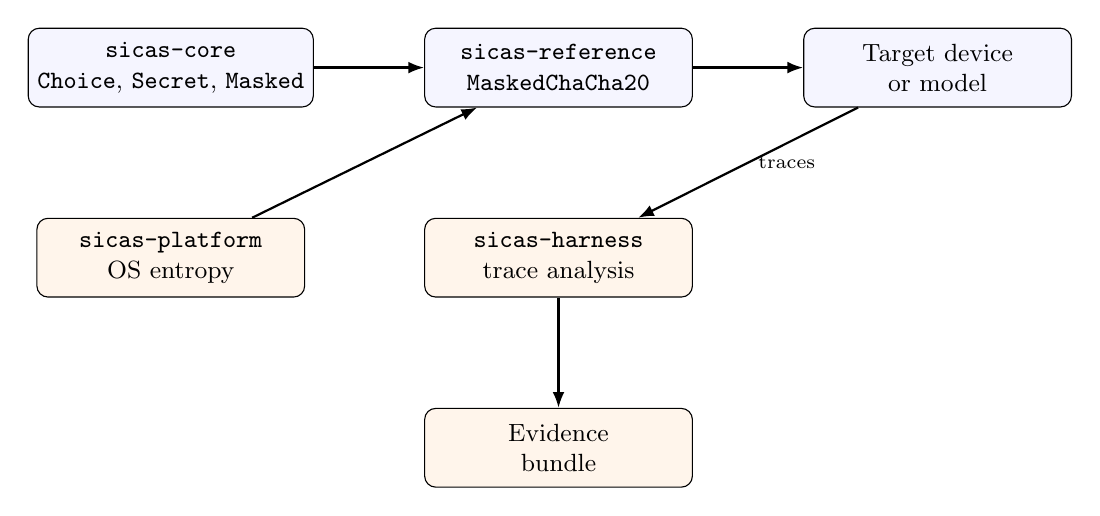
\begin{tikzpicture}[
  box/.style={draw, rounded corners, align=center, minimum width=34mm,
              minimum height=10mm, font=\small, fill=blue!4},
  tool/.style={draw, rounded corners, align=center, minimum width=34mm,
               minimum height=10mm, font=\small, fill=orange!8},
  arrow/.style={-{Latex[length=2mm]}, thick}
]
\node[box] (core) {\code{sicas-core}\\\code{Choice}, \code{Secret}, \code{Masked}};
\node[box, right=14mm of core] (ref) {\code{sicas-reference}\\\code{MaskedChaCha20}};
\node[box, right=14mm of ref] (target) {Target device\\or model};
\node[tool, below=14mm of core] (platform) {\code{sicas-platform}\\OS entropy};
\node[tool, below=14mm of ref] (harness) {\code{sicas-harness}\\trace analysis};
\node[tool, below=14mm of harness] (evidence) {Evidence\\bundle};
\draw[arrow] (core) -- (ref);
\draw[arrow] (platform) -- (ref);
\draw[arrow] (ref) -- (target);
\draw[arrow] (target) -- node[right, font=\scriptsize]{traces} (harness);
\draw[arrow] (harness) -- (evidence);
\end{tikzpicture}
\caption{SiCaS separates runtime building blocks from offline leakage assessment. The
reference integration is a validation target; the harness consumes traces and produces
evidence.}
\label{fig:architecture}
\end{figure}

The workspace contains five crates and a non-published fuzz crate:

\begin{description}[leftmargin=1.5em]
  \item[\code{sicas-core}] Constant-time primitives, \code{Secret<T>}, two-share
        \code{Masked<T>}, masked addition, and the fail-closed \code{EntropySource}
        trait. \code{no\_std}, \code{forbid(unsafe\_code)}, zero runtime dependencies.
  \item[\code{sicas-reference}] First-order masked ChaCha20. \code{no\_std},
        \code{forbid(unsafe\_code)}, zero runtime dependencies.
  \item[\code{sicas-harness}] Trace format, preprocessing, TVLA, CPA, DPA, timing,
        synthetic generation, leakage-model checks, and CLI. \code{std},
        \code{forbid(unsafe\_code)}, zero runtime dependencies.
  \item[\code{sicas-platform}] Safe OS entropy adapter. \code{std},
        \code{forbid(unsafe\_code)}, zero runtime dependencies. Unsupported platforms
        fail closed.
  \item[\code{sicas-zeroize}] Experimental volatile zeroization boundary.
        \code{no\_std}, isolated unsafe, non-published, unaudited, and not used by the
        published crates.
\end{description}

\subsection{Trust boundaries}

There are four explicit boundaries:

\begin{enumerate}[leftmargin=1.5em]
  \item \textbf{Entropy boundary.} The caller supplies an \code{EntropySource}. A
        failure must propagate as an error; there is no weak fallback.
  \item \textbf{Declassification boundary.} The declassification points are
        \code{Secret::expose\_secret},\allowbreak \code{Secret::into\_inner},\allowbreak
        \code{Masked::unmask},\allowbreak and the ChaCha20 keystream output. They expose
        plaintext values. They are documented and must be justified by
        the caller's leakage contract.
  \item \textbf{Device boundary.} The harness consumes traces from an external
        acquisition setup. It does not control the probe, the oscilloscope, or the
        target.
  \item \textbf{Release boundary.} The release manifest, SBOM, provenance, and signing
        dry run are separate from the runtime code. Production signing is not claimed.
\end{enumerate}

\subsection{Data flow}

A typical assessment is:

\begin{enumerate}[leftmargin=1.5em]
  \item acquire traces and plaintexts;
  \item serialise traces in the SiCaS binary format;
  \item trim, filter, and align;
  \item run TVLA, CPA, or DPA;
  \item publish the raw traces, parameters, tool versions, commit, and result.
\end{enumerate}

The harness never treats a passing test as a proof of absence of leakage. A result is
evidence for the tested target, trace count, leakage model, and acquisition setup.

\section{Masking and cryptographic design}\label{sec:design}

\subsection{Two-share masking}

\begin{definition}[Two-share Boolean sharing]\label{def:sharing}
For \(x\in\bits^n\), a two-share Boolean sharing is a pair
\((s_0,s_1)\in\bits^n\times\bits^n\) such that \(s_0\oplus s_1=x\). The sharing is
\emph{fresh} if the mask used to construct it is uniform and independent of \(x\) and
of all other masks.
\end{definition}

\begin{theorem}[Single-share uniformity]\label{thm:uniform}
Let \(r\) be uniform on \(\bits^n\) and independent of \(x\). Then
\(s_1=r\) and \(s_0=x\oplus r\) are each uniform on \(\bits^n\), and the marginal
distribution of either share is independent of \(x\).
\end{theorem}

\begin{proof}
For every \(y\in\bits^n\), \(\Prb[s_1=y]=2^{-n}\). For \(s_0\),
\(\Prb[s_0=y]=\Prb[r=y\oplus x]=2^{-n}\). The marginals do not depend on \(x\).
\end{proof}

This is the ideal first-order argument. It does not model glitches, transitions,
register reuse, or physical leakage that depends on both shares. Those effects are
outside the current claim and are why hardware validation remains necessary.

\subsection{Masked operations}

\begin{table}[htbp]
\centering
\caption{Masked operations and their correctness identities.}
\label{tab:masked-ops}
\begin{tabularx}{\linewidth}{@{}lX@{}}
\toprule
Operation & Identity / implementation \\
\midrule
XOR & \((a_0\oplus b_0,\;a_1\oplus b_1)\) \\
Complement & \((\neg a_0,\;a_1)\) \\
Refresh & \((a_0\oplus r,\;a_1\oplus r)\) with fresh \(r\) \\
AND & \(c_0=(a_0\wedge b_0)\oplus r\), \(c_1=(a_0\wedge b_1)\oplus(a_1\wedge b_0)\oplus(a_1\wedge b_1)\oplus r\) \\
Addition & ripple-carry over masked bits with a fresh mask per AND \\
Select & select each share independently with a public \code{Choice} \\
Equality & compare \(a_0\oplus b_0\) and \(a_1\oplus b_1\) in constant time \\
\bottomrule
\end{tabularx}
\end{table}

\begin{theorem}[Masked AND correctness]\label{thm:and}
For all \(a,b\in\bits^n\) and all shares \(a_0,a_1,b_0,b_1\) with
\(a_0\oplus a_1=a\) and \(b_0\oplus b_1=b\), the shares \(c_0,c_1\) in
Table~\ref{tab:masked-ops} satisfy \(c_0\oplus c_1=a\wedge b\).
\end{theorem}

\begin{proof}
Expand the four products:
\[
(a_0\oplus a_1)\wedge(b_0\oplus b_1)
= (a_0\wedge b_0)\oplus(a_0\wedge b_1)\oplus(a_1\wedge b_0)\oplus(a_1\wedge b_1).
\]
The two occurrences of \(r\) cancel under XOR.
\end{proof}

\begin{theorem}[Masked addition correctness]\label{thm:add}
For all \(a,b\in\bits^{32}\), the ripple-carry masked adder reconstructs
\((a+b)\bmod 2^{32}\).
\end{theorem}

\begin{proof}[Proof sketch]
At bit \(i\), the reconstructed sum bit is \(a_i\oplus b_i\oplus c_i\), and the
reconstructed carry is \((a_i\wedge b_i)\oplus(a_i\wedge c_i)\oplus(b_i\wedge c_i)\).
This is the standard full-adder identity. Induction on \(i\) from the zero carry gives
the 32-bit sum modulo \(2^{32}\). The masked AND gadgets preserve the reconstructed
values by Theorem~\ref{thm:and}, so the masked implementation computes the same function.
\end{proof}

The project's Kani harnesses check the core masked operations for all inputs of the
specified widths, including addition, refresh, selection, equality, and share
reconstruction. These are model-checking results for the Rust implementation, not a
mechanized proof of physical security.

\subsection{Masked ChaCha20}

The scalar masked ChaCha20 state is an array of sixteen \code{Masked<u32>} words. The
initial state is masked with fresh randomness. For each block, the working state and
the initial state used by the final addition are independently refreshed. This avoids
feeding correlated shares into the masked adder. The quarter round uses masked
addition, XOR, and rotation; the final addition uses the masked adder; the output is
unmasked only at the keystream boundary.

The bitsliced batch path processes 64 blocks at once. Each bit position of each 32-bit
word is represented by a \code{Masked<u64>} plane: the 64 bits of the plane correspond
to the 64 lanes. The quarter round is performed on planes; the masked adder is a
ripple-carry adder over the 32 bit planes. After the final addition, the planes are
transposed into 64 lane-major 64-byte blocks. The transpose is a 64$\times$64 bit-matrix
transpose implemented as a butterfly network with widths 32, 16, 8, 4, 2, and 1.

The bitsliced path is a performance optimisation, not a different security claim. It
uses the same two-share masking and fresh-mask discipline. Its output is validated
against the scalar and unmasked references, including counter wrap and batch/scalar
interoperability.

\subsection{Declassification and zeroization}

The following operations are declassification boundaries:

\begin{itemize}[leftmargin=1.5em]
  \item \code{Secret::expose\_secret} and \code{Secret::into\_inner};
  \item \code{Masked::unmask};
  \item the ChaCha20 keystream output;
  \item the bitsliced transpose, which unmasks the output planes before writing bytes.
\end{itemize}

The core and reference types do not guarantee zeroization on drop. The
\code{sicas-zeroize} crate is an experimental volatile-write boundary with a compiler
fence and a drop-path test. It is non-published, unaudited, and not integrated into the
published crates. A production zeroization claim would require an audited platform
adapter and a review of register, temporary, and move semantics.

\section{Leakage-assessment methodology}\label{sec:assessment}

\subsection{Trace format}

The trace format is deliberately small and strict:

\begin{verbatim}
magic:              8 bytes, b"SiCaSTR1"
version:            u16 little-endian, currently 1
samples_per_trace:  u32 little-endian
trace_count:        u32 little-endian
samples:            trace_count * samples_per_trace i16 little-endian
\end{verbatim}

The limits are \(10^6\) traces, \(10^6\) samples per trace, and \(10^8\) total samples.
The parser rejects invalid magic, unsupported versions, zero dimensions, ragged traces,
oversized inputs, and truncated files with typed errors. It is exercised by a
libFuzzer target and by Miri.

\subsection{Preprocessing}

\begin{description}[leftmargin=1.5em]
  \item[Trim.] Keep the half-open sample range \([s,e)\).
  \item[Filter.] Apply a centered moving average with a window of \(w\) samples and
        clipped edges. A window of one is the identity.
  \item[Align.] Choose the shift in \([-m,m]\) that maximises the normalized
        cross-correlation with a reference trace, then shift and zero-fill.
\end{description}

Preprocessing is part of the evidence. The parameters and the reference trace must be
published with the result.

\subsection{TVLA}

For each sample \(j\), let \(x_{0,j}\) and \(x_{1,j}\) be the fixed and random groups.
Welch's statistic is
\[
  t_j = \frac{\bar{x}_{0,j}-\bar{x}_{1,j}}
             {\sqrt{s_{0,j}^2/n_0+s_{1,j}^2/n_1}},
\]
where \(s^2\) is the sample variance. The implementation computes the statistic from
sums and sums of squares, clamps negative variances to zero, and reports the maximum
\(|t|\), its sample index, and the number of samples above the threshold. The default
threshold is \(4.5\).

TVLA is a detection test, not a proof of absence of leakage. A pass means that the
test did not detect a difference at the chosen threshold, trace count, and model.

\subsection{CPA}

For a key guess \(k\), plaintext \(p_i\), sample \(j\), and leakage model
\(M(k,p_i)\), CPA computes the Pearson correlation
\[
  \rho_{k,j} =
  \frac{\sum_i (M(k,p_i)-\bar{M}_k)(T_{i,j}-\bar{T}_j)}
       {\sqrt{\sum_i (M(k,p_i)-\bar{M}_k)^2
              \sum_i (T_{i,j}-\bar{T}_j)^2}}.
\]
The best key is the one with the largest absolute correlation across samples. The
default model is \(\HW(p_i\oplus k)\). The Hamming-weight model is invariant under key
complement: \(\HW(x\oplus k)\) and \(\HW(x\oplus k\oplus 0xFF)\) are perfectly
negatively correlated, so the tie-break returns the lower key. The library exposes
\code{cpa\_with\_model} for algorithm-specific models such as an AES S-box.

\subsection{DPA}

For each key guess \(k\), bit \(b\), and sample \(j\), partition the traces by
\[
  \Sbox[p_i\oplus k]_b.
\]
Let \(S_0\) and \(S_1\) be the two partitions. The difference of means is
\[
  \Delta_{k,b,j} =
  \frac{1}{|S_1|}\sum_{i\in S_1}T_{i,j}
  -
  \frac{1}{|S_0|}\sum_{i\in S_0}T_{i,j}.
\]
The report records the key, bit, sample, absolute difference, and signed difference of
the largest absolute difference. The search uses a strict \(>\) comparison, so the
first maximum wins.

The AES S-box supplies the nonlinearity that makes the partition key-dependent. A
single-bit partition may not uniquely recover the full key from noisy traces; several
bits or samples should be combined before treating a key as recovered. The synthetic
tests recover the exact key from noise-free single-bit leaks at bit 0 and bit 3,
including the sign of the difference.

\subsection{Timing and leakage-model checks}

The \code{timing} and \code{ct} commands run dudect-style fixed-vs-random tests
\citep{reparaz2017dudect} and report a \(t\)-statistic. The \code{leakage-check}
command measures the Pearson correlation between individual shares and the secret for
a masked byte, a masked AND composition, and a masked 32-bit addition. A negative
control correlates the secret with itself and must be detected. The command fails if
the control is missed or if any masked check exceeds the threshold.

These checks validate the masking model and the analysis code. They are not hardware
evidence and do not replace TVLA/CPA/DPA on a physical target.

\section{Security claims and evidence}\label{sec:claims}

\subsection{Claim taxonomy}

A claim is a statement about a property, a target, and a scope. The project uses three
categories:

\begin{enumerate}[leftmargin=1.5em]
  \item \textbf{Locally proven.} The claim has a test, proof, measurement, or
        reproducible evidence artifact in the repository.
  \item \textbf{Documented limitation.} The claim is not made; the limitation is
        recorded in the gap report.
  \item \textbf{External gate.} The claim requires hardware, credentials, or an
        independent party and is not simulated.
\end{enumerate}

\subsection{Claims C1--C10}

\begin{longtable}{@{}p{0.06\linewidth}p{0.42\linewidth}p{0.42\linewidth}@{}}
\caption{Claim matrix (abridged).}\label{tab:claims}\\
\toprule
ID & Claim & Current local status \\
\midrule
\endfirsthead
\toprule
ID & Claim & Current local status \\
\midrule
\endhead
C1 & The safe API prevents accidental secret-dependent branching/indexing. &
Compile-fail tests pass. \\
C2 & Constant-time gadgets are data-independent on supported targets. &
Dudect and assembly evidence pass on x86\_64; other targets pending. \\
C3 & First-order Boolean masking reduces first-order DPA below the TVLA threshold for
the reference algorithm. &
Synthetic and model evidence pass; hardware TVLA pending. \\
C4 & Entropy failure is fail-closed. &
Local fault tests pass; unsupported platforms return an error. \\
C5 & Zero runtime dependencies. &
Verified locally. \\
C6 & No unsafe code in core logic crates. &
\code{forbid(unsafe\_code)} verified locally. \\
C7 & Builds are reproducible. &
Verified locally across independent target directories. \\
C8 & Critical invariants are model-checked. &
30 Kani harnesses pass. \\
C9 & v1.0 meets SAL-4. &
Pending independent verification. \\
C10 & Release artifacts are signed and traceable. &
Local signing dry run only; production signing pending. \\
\bottomrule
\end{longtable}

\subsection{Proof obligations}

The proof obligations are maintained in \code{docs/PROOF\_OBLIGATIONS.md}. They cover
memory safety, functional correctness, constant-time behaviour, masking, entropy,
parser robustness, statistics, coverage, mutation, supply-chain integrity, release
integrity, and performance. Each obligation records the method, the evidence, and the
current status. A claim without an obligation is not part of the public claim set.

\subsection{Assurance levels}

\begin{table}[htbp]
\centering
\caption{SiCaS assurance levels.}
\label{tab:sal}
\begin{tabularx}{\linewidth}{@{}lXl@{}}
\toprule
Level & Requirements & Allowed public claim \\
\midrule
SAL-0 & Demo or prototype. & ``experimental'' \\
SAL-1 & Unit/integration tests and CI. & ``tested'' \\
SAL-2 & SAL-1 plus Miri, sanitizers, fuzzing, static analysis. & ``hardened'' \\
SAL-3 & SAL-2 plus formal/model checking, real-hardware TVLA, external audit. & ``audited'' \\
SAL-4 & SAL-3 plus independent red team, reproducible/signed builds, no open
critical/high findings, public evidence bundle. & ``SAL-4 under threat model T'' \\
\bottomrule
\end{tabularx}
\end{table}

The current label is \textbf{SAL-2 locally}. The project does not claim SAL-3 or SAL-4.

\section{Implementation and release engineering}\label{sec:implementation}

\subsection{Crate structure and API design}

The workspace uses Rust 2024 edition and MSRV 1.99. The shared workspace lints deny
\code{unsafe\_code}, missing docs, missing debug implementations, unreachable public
items, unused \code{must\_use}, and a set of Clippy pedantic and nursery lints. The
release profile uses \code{opt-level="z"}, fat LTO, one codegen unit,
\code{panic="abort"}, and stripped symbols.

The core API is intentionally small. \code{Secret<T>} does not implement
\code{PartialEq}, \code{Ord}, \code{Hash}, \code{Index}, \code{Clone}, or \code{Copy}.
This makes accidental equality, ordering, indexing, and copying a compile error.
\code{Masked<T>} exposes explicit share access only through documented methods.
\code{EntropySource} returns \code{Result}; there is no weak fallback.

\subsection{Fail-closed entropy}

The \code{sicas-platform} adapter reads \code{/dev/urandom} on Unix-like systems. If
the source cannot be opened, it returns \code{EntropyError::Unavailable}. Other
platforms return the same error until a dedicated adapter is added. The core
\code{EntropySource} trait requires implementations to fill the destination completely
or return an error; partial fill followed by success is a contract violation.

\subsection{Constant-time discipline}

The constant-time claim is supported by three layers:

\begin{enumerate}[leftmargin=1.5em]
  \item branchless formulas in the core gadgets;
  \item assembly inspection across optimization levels, codegen units, panic
        strategies, and LTO variants;
  \item dudect-style timing tests on x86\_64.
\end{enumerate}

The assembly checker covers 69 configurations: opt-level 0 on four targets,
opt-levels 0/1/2/3/s and codegen/panic variants on x86\_64 and AArch64, and thin/fat
LTO on x86\_64. The dudect evidence includes \(5\times10^6\) debug-profile samples and
\(3\times10^6\) release-profile samples per check. These are local measurements; they
do not cover every compiler, CPU, or physical target.

\subsection{Release and supply chain}

The release manifest script builds the workspace, copies \code{sicas-harness}, and
writes a SHA-256 checksum, a CycloneDX SBOM \citep{cyclonedx}, and provenance metadata.
The manifest validator checks the artifact hash, checksum file, provenance, SBOM
component graph, workspace versions, timestamp, and (optionally) the current commit.
The local signing dry run produces and verifies a detached signature with an ephemeral
test key. It is a process check, not a production identity.

The release binary for the current package is 386{,}232 bytes with SHA-256:
\begin{center}\small
\code{1f0d304ca9b9582fd9153e7c006c240bd0e06acc3a685dfad93088429e4de7da}
\end{center}
The release build commit is \code{123eb69}; the proof code commit is \code{ef13675}.
The binary is reproducible across independent target directories.

\section{Evaluation}\label{sec:evaluation}

\subsection{Functional correctness}

The workspace passes its unit, integration, property, and doctest suites. The core
tests cover constant-time comparison, selection, swap, lookup, secret handling, masking,
refresh, share reconstruction, and masked addition. The reference tests cover RFC~8439
vectors, differential checks against an unmasked reference, lane-independent bitsliced
addition, key-plane balance, batch/scalar interoperability, counter wrap, and
entropy-failure propagation. The harness tests cover trace parsing, preprocessing,
TVLA, CPA, DPA, timing validation, synthetic generation, and leakage-model checks.

\subsection{Memory safety and undefined behaviour}

Miri \citep{miri} is run over the workspace, with reduced iteration counts and
documented skips for native-only statistical, OS, and subprocess paths. AddressSanitizer
\citep{serebryany2012asan} runs over the workspace library tests. Valgrind
\citep{nethercote2007valgrind} runs over five library test binaries with
\code{--leak-check=full} and \code{--errors-for-leak-kinds=definite}. All three report
no errors on the covered paths.

\subsection{Model checking}

Kani \citep{kani} is used for 30 harnesses covering constant-time gadgets, masked linear
and logical operations, addition, refresh, selection, equality, share reconstruction,
and share uniformity. The proofs are bounded to the declared widths and assumptions;
they are not a proof of physical security.

\subsection{Mutation, coverage, and fuzzing}

The current workspace mutation run tests 630 mutants: 574 are caught, 0 are missed, and
56 are unviable. The DPA file is also mutated in a targeted run: 30 mutants, 29 caught,
0 missed, 1 unviable. Line coverage is 97.28\% and region coverage is 94.89\%; the DPA
module is at 100\% line coverage. Five libFuzzer campaigns cover masked operations,
constant-time lookup, trace parsing, ChaCha20, and the bitsliced batch path at one
million executions each.

\subsection{Cross-architecture and performance}

AArch64 Linux under QEMU passes 141 workspace library tests; i686 native passes 154
all-target tests. The bitsliced masked ChaCha20 batch measures 7.15$\times$ versus the
unmasked reference in the final full proof, meeting the 10$\times$ hard ceiling. The
5$\times$ target remains open; reaching it requires SIMD or a faster audited mask
stream, both of which would create a new security boundary.

\subsection{Summary}

\begin{table}[htbp]
\centering
\caption{Local evidence summary.}
\label{tab:evidence}
\begin{tabularx}{\linewidth}{@{}lX@{}}
\toprule
Gate & Result \\
\midrule
Full local proof & PASS at \code{8c41e4b} \\
AES S-box DPA quick proof & PASS at \code{ef13675} \\
ASan & 141 workspace library tests pass \\
Kani & 30 harnesses pass \\
Mutation & 630 mutants, 574 caught, 0 missed, 56 unviable \\
Coverage & 97.28\% lines, 94.89\% regions \\
Fuzzing & Five 1M-execution campaigns \\
AArch64 QEMU / i686 & 141 / 154 tests pass \\
Valgrind & Five binaries, zero errors \\
Release & 386{,}232 bytes, reproducible, validator and signing dry run pass \\
Evidence bundle & 109 files, hashes verified \\
\bottomrule
\end{tabularx}
\end{table}

\section{Limitations and open gaps}\label{sec:limitations}

\subsection{No hardware leakage evidence}

The project has no physical power or electromagnetic traces. The synthetic and
model-based evidence validates the analysis path and the masking construction, but it
does not prove that a device leaks less. Hardware TVLA/CPA/DPA remains the central
external gate.

\subsection{No independent audit or red team}

The local self-audit and adversarial review are useful, but they are not independent.
An external audit and an independent red team are required before SAL-3/SAL-4.

\subsection{Higher-order, fault, and invasive attacks}

The masking is first-order. It does not claim security against higher-order DPA,
fault injection, invasive probing, cache-timing, or microarchitectural attacks.

\subsection{Template attacks}

Profiling template attacks are outside the threat model. The harness includes DPA, but
not a template-attack implementation. This is a scope decision, not a claim that
template attacks are infeasible.

\subsection{Performance gap}

The 10$\times$ hard ceiling is met; the 5$\times$ target is open. The remaining gap is
in the bitsliced masked adder and entropy stream. SIMD or a faster audited mask stream
would require a new proof.

\subsection{Zeroization}

The experimental zeroization adapter is not a production guarantee. It is
non-published, unaudited, and not integrated into the published crates. A production
claim requires an audited boundary and a review of register, temporary, and move
semantics.

\subsection{Platform coverage}

The core and reference crates are \code{no\_std} and compile for embedded targets, but
runtime evidence is limited to x86\_64, AArch64 QEMU, and i686. ARM/RISC-V runtime
timing and hardware leakage remain pending. Windows, macOS, iOS, Android, eBPF, and
kernel modules are not supported in v1.0.

\section{Roadmap to SAL-4}\label{sec:roadmap}

The roadmap separates local work from external gates.

\begin{enumerate}[leftmargin=1.5em]
  \item \textbf{Freeze the local proof.} The current package is the audit-ready local
        artifact. Any code change requires a new proof run and a new evidence bundle.
  \item \textbf{Independent audit.} An external auditor reviews the threat model,
        claims, code, tests, and evidence, and reports findings.
  \item \textbf{Independent red team.} A red team attempts to break the claims with
        implementation, statistical, and physical attacks.
  \item \textbf{Hardware validation.} Acquire power/EM traces from physical targets and
        run TVLA/CPA/DPA with published parameters and raw data.
  \item \textbf{Production signing.} Replace the ephemeral signing dry run with a
        production identity and a real Sigstore/SLSA release run.
  \item \textbf{Remediation and retest.} Fix findings, rerun the gates, and publish the
        updated evidence.
  \item \textbf{SAL-4 decision.} Claim SAL-4 only when every criterion is met and
        independently verified.
\end{enumerate}

Optional local work includes SIMD for the 5$\times$ target, template-attack tooling,
Kani coverage for the bitsliced adder, and a reviewed zeroization adapter. These are
enhancements, not substitutes for the external gates.

\section{Related work}\label{sec:related}

Timing attacks \citep{kocher1996timing}, DPA \citep{kocher1999dpa}, CPA
\citep{brier2004cpa}, and template attacks \citep{chari2002template} established the
main side-channel analysis families. \citet{mangard2007power} provide a comprehensive
treatment of power analysis and countermeasures. Private circuits
\citep{ishai2003private}, threshold implementations \citep{nikova2006threshold}, and
probing-secure masking \citep{rivain2010probing} provide the theoretical background for
masking. TVLA \citep{goodwill2011tvla,schneider2015leakage} and ISO/IEC~17825
\citep{iso17825} provide evaluation methodologies. Dudect
\citep{reparaz2017dudect} provides a practical constant-time test.

On the implementation side, RustBelt \citep{jung2018rustbelt} provides a formal
foundation for Rust safety, Kani \citep{kani} provides bounded model checking, libFuzzer
\citep{libfuzzer} provides coverage-guided fuzzing, and mutation testing
\citep{jia2011mutation} measures test-suite strength. Release integrity is informed by
SLSA \citep{slsa}, Sigstore \citep{sigstore}, and CycloneDX \citep{cyclonedx}. FIPS~197
\citep{fips197} defines AES, RFC~8439 \citep{rfc8439} defines ChaCha20 and Poly1305,
and \citet{bernstein2008chacha} introduced ChaCha. NIST SP~800-90A
\citep{nist80090a} and FIPS~140-3 \citep{fips1403} provide context for entropy and
module security, although SiCaS does not claim FIPS certification.

SiCaS differs from a pure library or a pure evaluation tool by combining a masked
reference integration with an assessment harness and an evidence system in one
workspace. It is intentionally narrower than a general-purpose cryptographic library
and intentionally more rigorous than a benchmark suite.

\section{Conclusion}\label{sec:conclusion}

SiCaS is a local-first, evidence-first engineering package for first-order side-channel
attenuation and leakage assessment. It provides safe-Rust masked primitives, a masked
ChaCha20 reference integration, a zero-dependency assessment harness, and a reproducible
evidence bundle. The current label is SAL-2 locally. The 10$\times$ performance hard
ceiling is met; the 5$\times$ target is open. The package is ready for independent
review, not for production use. The next meaningful step is external verification:
audit, red team, hardware leakage measurement, and production signing.

\appendix

\section{Glossary}

\begin{description}[leftmargin=1.5em]
  \item[CPA] Correlation power analysis.
  \item[DPA] Differential power analysis.
  \item[EM] Electromagnetic.
  \item[LTO] Link-time optimisation.
  \item[MSRV] Minimum supported Rust version.
  \item[SAL] SiCaS assurance level.
  \item[SBOM] Software bill of materials.
  \item[TVLA] Test Vector Leakage Assessment.
\end{description}

\section{Claim-to-evidence matrix}

\begin{longtable}{@{}p{0.08\linewidth}p{0.44\linewidth}p{0.40\linewidth}@{}}
\caption{Claim-to-evidence map.}\label{tab:claim-evidence}\\
\toprule
Claim & Evidence & Status \\
\midrule
\endfirsthead
\toprule
Claim & Evidence & Status \\
\midrule
\endhead
C1 & Compile-fail doctests for \code{Secret}. & Pass \\
C2 & Dudect and 69-configuration assembly matrix. & Pass on x86\_64 \\
C3 & Synthetic TVLA/CPA/DPA, leakage model, bitsliced differential tests. & Local pass; hardware pending \\
C4 & Entropy failure tests; Unix adapter; unsupported platforms fail closed. & Pass \\
C5 & \code{cargo metadata} zero-dependency check. & Pass \\
C6 & \code{forbid(unsafe\_code)} in core, reference, platform, harness. & Pass \\
C7 & Two-build hash comparison. & Pass \\
C8 & 30 Kani harnesses. & Pass \\
C9 & Independent verification of every SAL-4 criterion. & Pending \\
C10 & Manifest, SBOM, provenance, signing dry run. & Local pass; production pending \\
\bottomrule
\end{longtable}

\section{Reproducibility commands}

\begin{verbatim}
cargo build --workspace --release --locked
cargo test --workspace --all-targets --all-features --locked
cargo test --workspace --doc --locked
./tools/local_proof.sh quick
./tools/local_proof.sh full

cd evidence/bundle
sha256sum -c MANIFEST.sha256

python3 tools/validate_release_manifest.py \
  --manifest evidence/release/2026-10-31-sbox-dpa --skip-commit

cd evidence/release/2026-10-31-sbox-dpa
sha256sum -c SHA256SUMS
\end{verbatim}

\section{Document history}

\small
\begin{longtable}{@{}p{0.12\linewidth}p{0.18\linewidth}p{0.24\linewidth}p{0.38\linewidth}@{}}
\caption{White paper revision history.}\label{tab:history}\\
\toprule
Version & Date & Code / evidence & Changes \\
\midrule
\endfirsthead
\toprule
Version & Date & Code / evidence & Changes \\
\midrule
\endhead
0.1.0 & 2026-10-30 & initial tree & Problem statement, threat model, architecture outline. \\
0.9.0 & 2026-10-31 & \code{8c41e4b} & Full local proof, evaluation chapter, evidence summary. \\
1.0.0 & 2026-10-31 & \code{ef13675}, \evidencetag & AES S-box DPA, GPL-3.0-only, audit-ready package. \\
\bottomrule
\end{longtable}

\bibliographystyle{plainnat}
\bibliography{../references}

\end{document}
